\begin{frame}{Database generation strategy}
    \newcommand\WIDTH{3.5cm}
    \newcommand\HEIGHT{1.5cm}
    \newcommand\Ydist{2cm}
    \newcommand\XPOS{4cm}
    \newcommand\TOTheight{5cm}
    \newcommand\TOTwidth{6cm}
    \newcommand\PTS{2pt}
    \newcommand\xSpace{0.5cm}

    \only<1>{
        \begin{figure}
            \centering
            \vspace*{0.5cm}
            \hspace*{0.3cm}
            \begin{tikzpicture}
    
    \node[draw,
        rectangle,
        text centered,
        line width = \PTS,
        minimum height = \TOTheight,
        minimum width = \TOTwidth
    ] (optimizationProcess) at (0, 0) {\large{\textbf{Optimization}}};

    % \node[
    %     below right = 0.5cm and 0.5cm of optimizationProcess.north west 
    % ] {
    %     
\includegraphics[scale=0.08]{./MITlogo.png}
    % };

    % \node[
    %     above left = 0.15cm and 0.5cm of optimizationProcess.south east 
    % ] {
    %     
\includegraphics[scale=0.3]{./SCIPYlogo.png}
    % };

    \node[draw,
        rectangle,
        text centered,
        line width = \PTS,
        % minimum width = \WIDTH,
        minimum height = \HEIGHT,
        right = 2*\xSpace of optimizationProcess
    ] (database) {\large{\textbf{Database}}};
    
    \coordinate[left=\xSpace of optimizationProcess.west]  (c1) {};
    \coordinate[above=\Ydist of c1]                      (c2) {};
    \coordinate[below=\Ydist of c1]                      (c3) {};

    \node[draw,
        rectangle,
        text centered,
        line width = \PTS,
        minimum width = \WIDTH,
        minimum height = \HEIGHT,
        left = \xSpace of c2
    ] (designSpace) {\large{\textbf{\makecell[c]{Design space\\reduction}}}};

    \node[draw,
        rectangle,
        text centered,
        line width = \PTS,
        minimum width = \WIDTH,
        minimum height = \HEIGHT,
        left = \xSpace of c1
    ] (constr) {\large{\textbf{Constraints}}};

    \node[draw,
        rectangle,
        text centered,
        line width = \PTS,
        minimum width = \WIDTH,
        minimum height = \HEIGHT,
        left = \xSpace of c3
    ] (obj) {\large{\textbf{Objectives}}};

    \draw[-latex, line width = 1pt] (designSpace) -- (c2) -- (c1) to (optimizationProcess.west);
    \draw[-latex, line width = 1pt] (constr) to (optimizationProcess.west);
    \draw[-latex, line width = 1pt] (obj) -- (c3) -- (c1) to (optimizationProcess.west);
    \draw[-latex, line width = 1pt] (optimizationProcess.east) to (database.west);

\end{tikzpicture}
            % 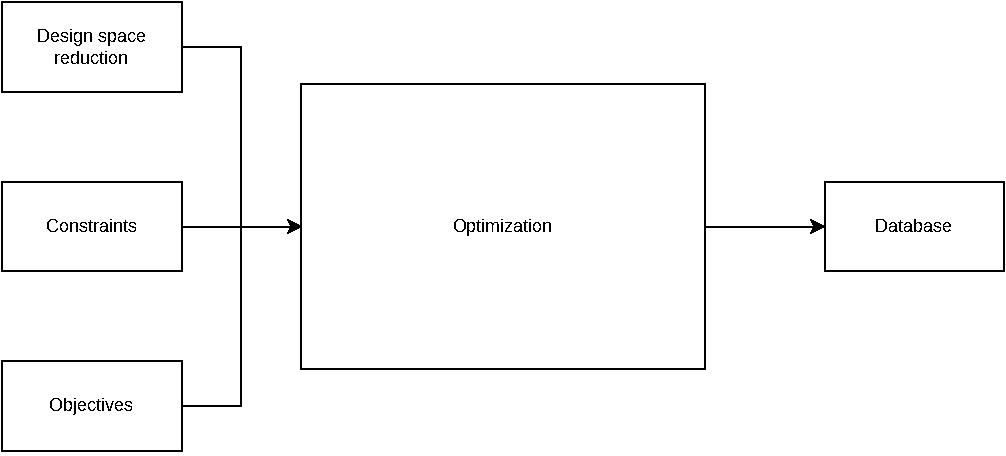
\includegraphics[page=1, scale=0.7]{pdf/databaseScheme-start.drawio}
        \end{figure}
    }
    \only<2>{
        \begin{figure}
            \centering
            \vspace*{0.5cm}
            \hspace*{0.3cm}
            \begin{tikzpicture}
    
    \node[draw,
        rectangle,
        text centered,
        line width = \PTS,
        minimum height = \TOTheight,
        minimum width = \TOTwidth
    ] (optimizationProcess) at (0, 0) {\large{\textbf{Optimization}}};

    % \node[
    %     below right = 0.5cm and 0.5cm of optimizationProcess.north west 
    % ] {
    %     
\includegraphics[scale=0.08]{./MITlogo.png}
    % };

    % \node[
    %     above left = 0.15cm and 0.5cm of optimizationProcess.south east 
    % ] {
    %     
\includegraphics[scale=0.3]{./SCIPYlogo.png}
    % };

    \node[draw,
        rectangle,
        text centered,
        line width = \PTS,
        % minimum width = \WIDTH,
        minimum height = \HEIGHT,
        right = 2*\xSpace of optimizationProcess
    ] (database) {\large{\textbf{Database}}};
    
    \coordinate[left=\xSpace of optimizationProcess.west]  (c1) {};
    \coordinate[above=\Ydist of c1]                      (c2) {};
    \coordinate[below=\Ydist of c1]                      (c3) {};

    \node[draw,
        rectangle,
        text centered,
        line width = \PTS,
        minimum width = \WIDTH,
        minimum height = \HEIGHT,
        left = \xSpace of c2
    ] (designSpace) {\large{\textbf{\makecell[c]{Kulfan\\parametrization}}}};

    \node[draw,
        rectangle,
        text centered,
        line width = \PTS,
        minimum width = \WIDTH,
        minimum height = \HEIGHT,
        left = \xSpace of c1
    ] (constr) {\large{\textbf{Constraints}}};

    \node[draw,
        rectangle,
        text centered,
        line width = \PTS,
        minimum width = \WIDTH,
        minimum height = \HEIGHT,
        left = \xSpace of c3
    ] (obj) {\large{\textbf{Objectives}}};

    \draw[-latex, line width = 1pt] (designSpace) -- (c2) -- (c1) to (optimizationProcess.west);
    \draw[-latex, line width = 1pt] (constr) to (optimizationProcess.west);
    \draw[-latex, line width = 1pt] (obj) -- (c3) -- (c1) to (optimizationProcess.west);
    \draw[-latex, line width = 1pt] (optimizationProcess.east) to (database.west);

\end{tikzpicture}
            % 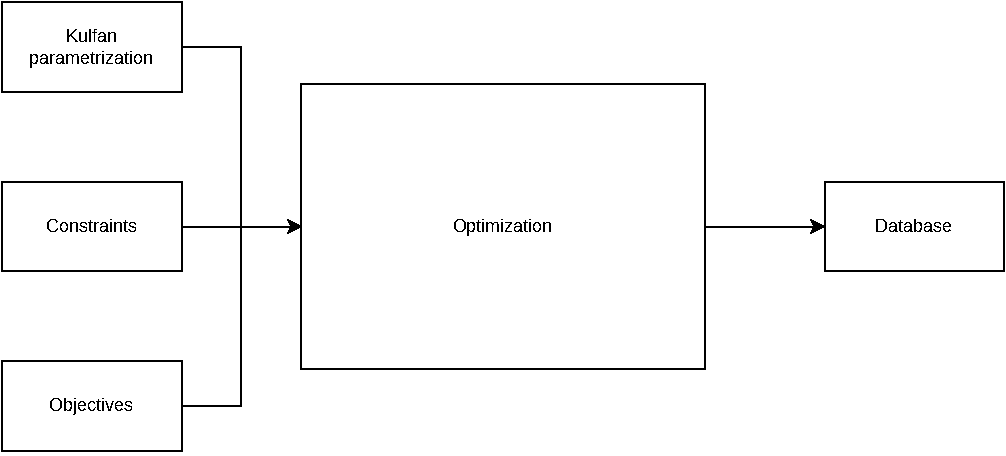
\includegraphics[page=1, scale=0.7]{pdf/databaseScheme-kulfan.drawio}
        \end{figure}
    }
    \only<3>{
        \begin{figure}
            \centering
            \vspace*{0.5cm}
            \hspace*{0.3cm}
            \begin{tikzpicture}
    
    \node[draw,
        rectangle,
        text centered,
        line width = \PTS,
        minimum height = \TOTheight,
        minimum width = \TOTwidth
    ] (optimizationProcess) at (0, 0) {\large{\textbf{Optimization}}};

    % \node[
    %     below right = 0.5cm and 0.5cm of optimizationProcess.north west 
    % ] {
    %     
\includegraphics[scale=0.08]{./MITlogo.png}
    % };

    % \node[
    %     above left = 0.15cm and 0.5cm of optimizationProcess.south east 
    % ] {
    %     
\includegraphics[scale=0.3]{./SCIPYlogo.png}
    % };

    \node[draw,
        rectangle,
        text centered,
        line width = \PTS,
        % minimum width = \WIDTH,
        minimum height = \HEIGHT,
        right = 2*\xSpace of optimizationProcess
    ] (database) {\large{\textbf{Database}}};
    
    \coordinate[left=\xSpace of optimizationProcess.west]  (c1) {};
    \coordinate[above=\Ydist of c1]                      (c2) {};
    \coordinate[below=\Ydist of c1]                      (c3) {};

    \node[draw,
        rectangle,
        text centered,
        line width = \PTS,
        minimum width = \WIDTH,
        minimum height = \HEIGHT,
        left = \xSpace of c2
    ] (designSpace) {\large{\textbf{\makecell[c]{Kulfan\\parametrization}}}};

    \node[draw,
        rectangle,
        text centered,
        line width = \PTS,
        minimum width = \WIDTH,
        minimum height = \HEIGHT,
        left = \xSpace of c1
    ] (constr) {\large{\textbf{\makecell[c]{Aerodynamic\\Duty}}}};

    \node[draw,
        rectangle,
        text centered,
        line width = \PTS,
        minimum width = \WIDTH,
        minimum height = \HEIGHT,
        left = \xSpace of c3
    ] (obj) {\large{\textbf{Objectives}}};

    \draw[-latex, line width = 1pt] (designSpace) -- (c2) -- (c1) to (optimizationProcess.west);
    \draw[-latex, line width = 1pt] (constr) to (optimizationProcess.west);
    \draw[-latex, line width = 1pt] (obj) -- (c3) -- (c1) to (optimizationProcess.west);
    \draw[-latex, line width = 1pt] (optimizationProcess.east) to (database.west);

\end{tikzpicture}
            % 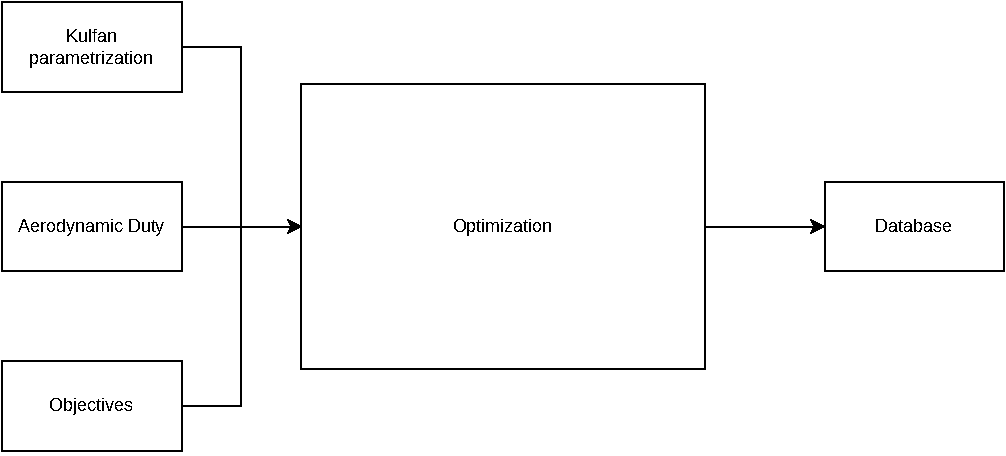
\includegraphics[page=1, scale=0.7]{pdf/databaseScheme-aerodynamicDuty.drawio}
        \end{figure}
    }
    \only<4>{
        \begin{figure}
            \centering
            \vspace*{0.5cm}
            \hspace*{0.3cm}
            \begin{tikzpicture}
    
    \node[draw,
        rectangle,
        text centered,
        line width = \PTS,
        minimum height = \TOTheight,
        minimum width = \TOTwidth
    ] (optimizationProcess) at (0, 0) {\large{\textbf{Optimization}}};

    % \node[
    %     below right = 0.5cm and 0.5cm of optimizationProcess.north west 
    % ] {
    %     
\includegraphics[scale=0.08]{./MITlogo.png}
    % };

    % \node[
    %     above left = 0.15cm and 0.5cm of optimizationProcess.south east 
    % ] {
    %     
\includegraphics[scale=0.3]{./SCIPYlogo.png}
    % };

    \node[draw,
        rectangle,
        text centered,
        line width = \PTS,
        % minimum width = \WIDTH,
        minimum height = \HEIGHT,
        right = 2*\xSpace of optimizationProcess
    ] (database) {\large{\textbf{Database}}};
    
    \coordinate[left=\xSpace of optimizationProcess.west]  (c1) {};
    \coordinate[above=\Ydist of c1]                      (c2) {};
    \coordinate[below=\Ydist of c1]                      (c3) {};

    \node[draw,
        rectangle,
        text centered,
        line width = \PTS,
        minimum width = \WIDTH,
        minimum height = \HEIGHT,
        left = \xSpace of c2
    ] (designSpace) {\large{\textbf{\makecell[c]{Kulfan\\parametrization}}}};

    \node[draw,
        rectangle,
        text centered,
        line width = \PTS,
        minimum width = \WIDTH,
        minimum height = \HEIGHT,
        left = \xSpace of c1
    ] (constr) {\large{\textbf{\makecell[c]{Aerodynamic\\Duty}}}};

    \node[draw,
        rectangle,
        text centered,
        line width = \PTS,
        minimum width = \WIDTH,
        minimum height = \HEIGHT,
        left = \xSpace of c3
    ] (obj) {\large{\textbf{\makecell[c]{Aerodynamic\\Style}}}};

    \draw[-latex, line width = 1pt] (designSpace) -- (c2) -- (c1) to (optimizationProcess.west);
    \draw[-latex, line width = 1pt] (constr) to (optimizationProcess.west);
    \draw[-latex, line width = 1pt] (obj) -- (c3) -- (c1) to (optimizationProcess.west);
    \draw[-latex, line width = 1pt] (optimizationProcess.east) to (database.west);

\end{tikzpicture}
            % 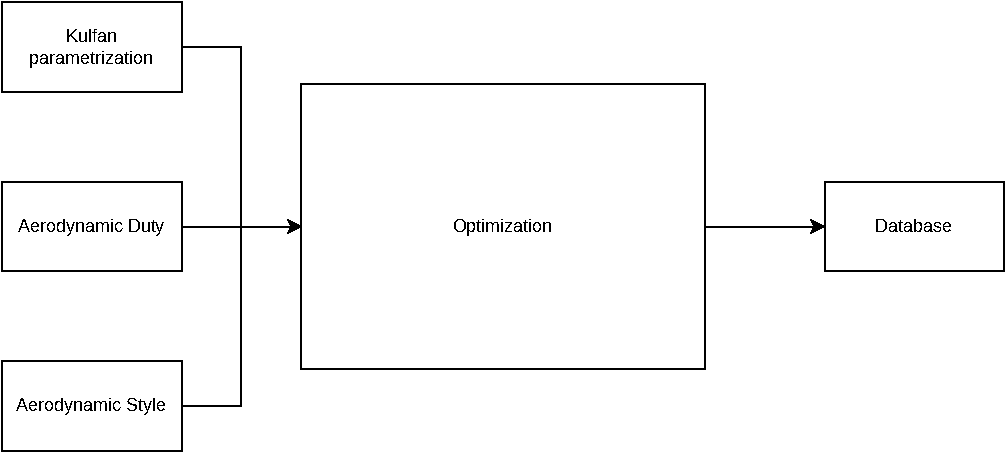
\includegraphics[page=1, scale=0.7]{pdf/databaseScheme-aerodynamicStyle.drawio}
        \end{figure}
    }
    \only<5>{
        \begin{figure}
            \centering
            \vspace*{0.5cm}
            \hspace*{0.3cm}
            \begin{tikzpicture}
    
    \node[draw,
        rectangle,
        text centered,
        line width = \PTS,
        minimum height = \TOTheight,
        minimum width = \TOTwidth
    ] (optimizationProcess) at (0, 0) {};

    \node[
        below right = 0.25cm and 0.25cm of optimizationProcess.north west 
    ] {
        
\includegraphics[scale=0.05]{./images/MITlogo.png}
    };

    \node[
        above left = 0.02cm and 0.02cm of optimizationProcess.south east 
    ] {
        
\includegraphics[scale=0.2]{./images/SCIPYlogo.png}
    };

    \node[draw,
        rectangle,
        text centered,
        line width = \PTS,
        % minimum width = 2cm,
        minimum height = \HEIGHT,
        right = 2*\xSpace of optimizationProcess
    ] (database) {\large{\textbf{Database}}};
    
    \coordinate[left=\xSpace of optimizationProcess.west]  (c1) {};
    \coordinate[above=\Ydist of c1]                      (c2) {};
    \coordinate[below=\Ydist of c1]                      (c3) {};

    \node[draw,
        rectangle,
        text centered,
        line width = \PTS,
        minimum width = \WIDTH,
        minimum height = \HEIGHT,
        left = \xSpace of c2
    ] (designSpace) {\large{\textbf{\makecell[c]{Kulfan\\parametrization}}}};

    \node[draw,
        rectangle,
        text centered,
        line width = \PTS,
        minimum width = \WIDTH,
        minimum height = \HEIGHT,
        left = \xSpace of c1
    ] (constr) {\large{\textbf{\makecell[c]{Aerodynamic\\Duty}}}};

    \node[draw,
        rectangle,
        text centered,
        line width = \PTS,
        minimum width = \WIDTH,
        minimum height = \HEIGHT,
        left = \xSpace of c3
    ] (obj) {\large{\textbf{\makecell[c]{Aerodynamic\\Style}}}};

    \draw[-latex, line width = 1pt] (designSpace) -- (c2) -- (c1) to (optimizationProcess.west);
    \draw[-latex, line width = 1pt] (constr) to (optimizationProcess.west);
    \draw[-latex, line width = 1pt] (obj) -- (c3) -- (c1) to (optimizationProcess.west);
    \draw[-latex, line width = 1pt] (optimizationProcess.east) to (database.west);

\end{tikzpicture}
            % 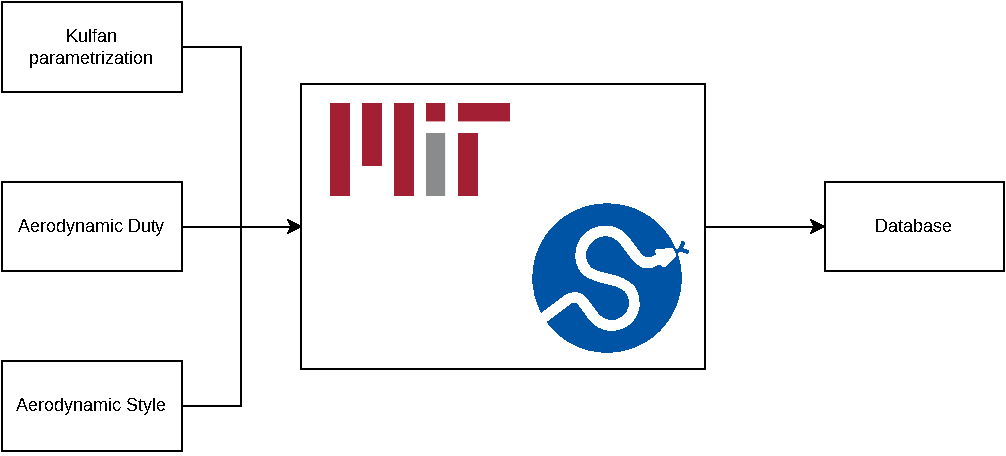
\includegraphics[page=1, scale=0.7]{pdf/databaseScheme-optimization.drawio}
        \end{figure}
    }
\end{frame}

\begin{frame}{Database points}
    \only<1>{
        \begin{columns}
            \column{0.5\textwidth}
            \begin{figure}
                \centering
                % \hspace*{-1cm}
                % \vspace{1cm}
                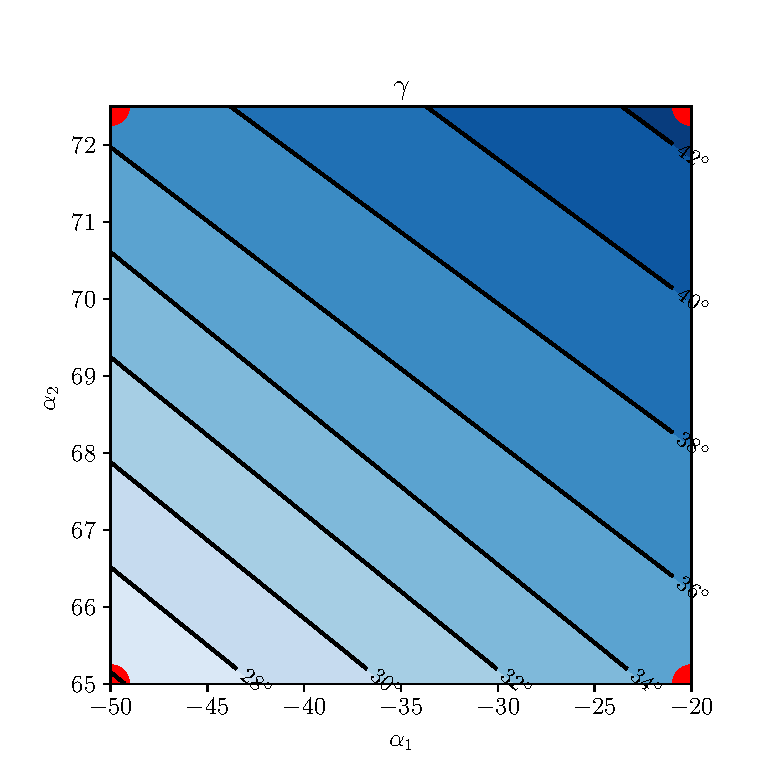
\includegraphics[scale=0.5]{images/staggerLinear.eps}
            \end{figure}
            \column{0.5\textwidth}
            \begin{itemize}
                \item Data optimization \textbf{starting from the boundaries of the domain} of study
                % \item From the \textbf{corner points} of the domain, it is \textbf{computed a new guess} for the optimization of the inner points
                % \item The new guess is made using a \textbf{linear interpolation} of optimized data 
                % \item Once this procedure generates \textbf{sufficient data for the ML training}, data collection is stopped
            \end{itemize}
        \end{columns}
    }
    \only<2>{
        \begin{columns}
            \column{0.5\textwidth}
            \begin{figure}
                \centering
                % \hspace*{-1cm}
                % \vspace{1cm}
                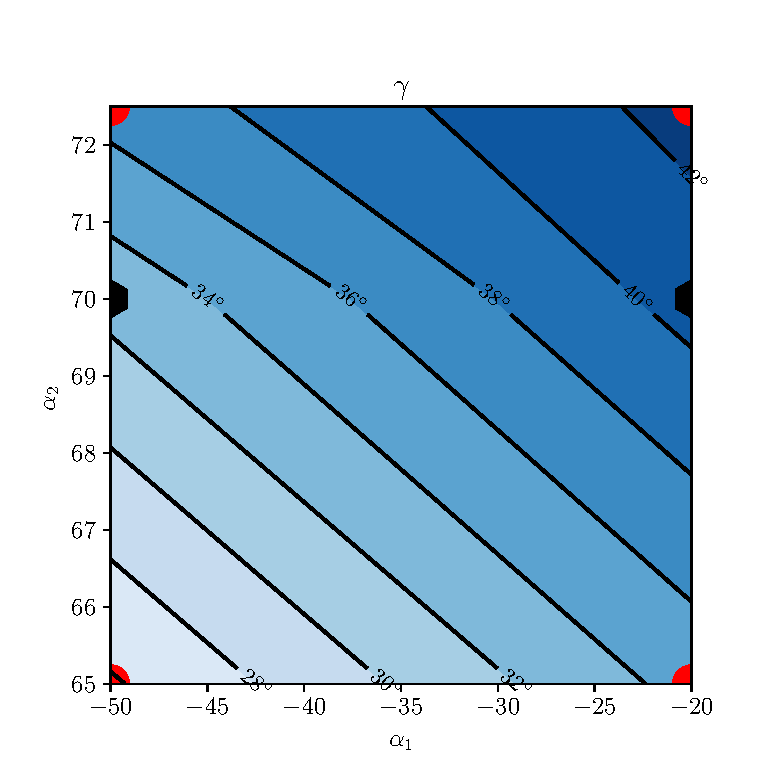
\includegraphics[scale=0.5]{images/staggerLinear1.eps}
            \end{figure}
            \column{0.5\textwidth}
            \begin{itemize}
                \item Data optimization \textbf{starting from the boundaries of the domain} of study
                \item From the \textbf{corner points} of the domain, it is \textbf{computed a new guess} for the optimization of the inner points
                \item The new guess is made using a \textbf{linear interpolation} of optimized data 
                % \item Once this procedure generates \textbf{sufficient data for the ML training}, data collection is stopped
            \end{itemize}
        \end{columns}
    }
    \only<3>{
        \begin{columns}
            \column{0.5\textwidth}
            \begin{figure}
                \centering
                % \hspace*{-1cm}
                % \vspace{1cm}
                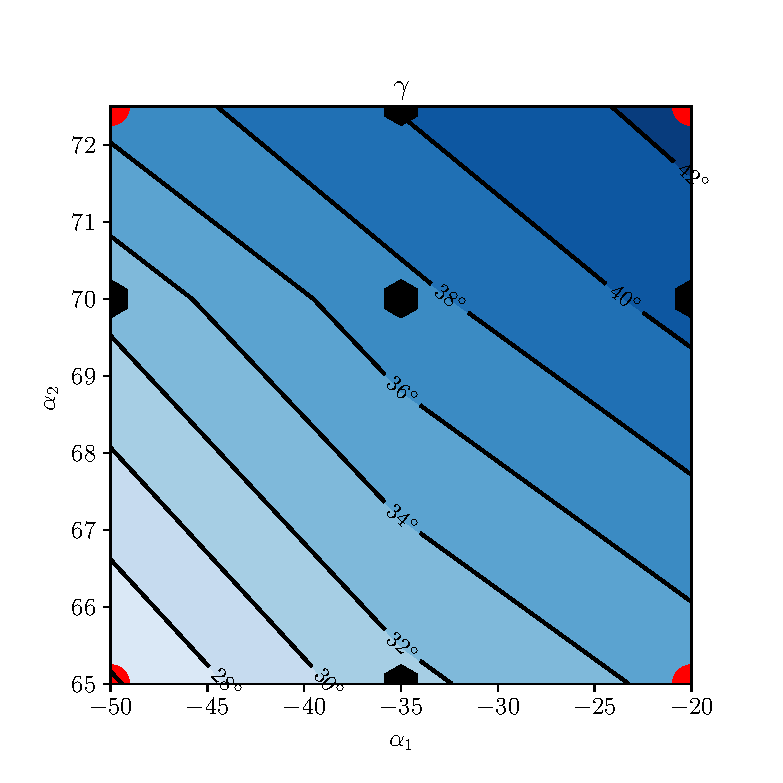
\includegraphics[scale=0.5]{images/staggerLinear2.eps}
            \end{figure}
            \column{0.5\textwidth}
            \begin{itemize}
                \item Data optimization \textbf{starting from the boundaries of the domain} of study
                \item From the \textbf{corner points} of the domain, it is \textbf{computed a new guess} for the optimization of the inner points
                \item The new guess is made using a \textbf{linear interpolation} of optimized data 
                % \item Once this procedure generates \textbf{sufficient data for the ML training}, data collection is stopped
            \end{itemize}
        \end{columns}
    }
    \only<4>{
        \begin{columns}
            \column{0.5\textwidth}
            \begin{figure}
                \centering
                % \hspace*{-1cm}
                % \vspace{1cm}
                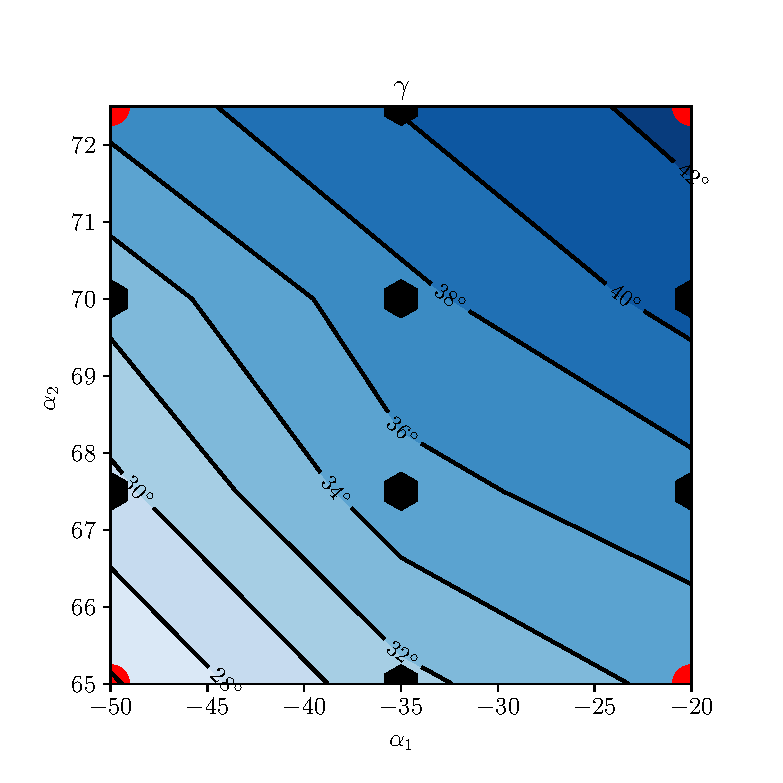
\includegraphics[scale=0.5]{images/staggerComplete.eps}
            \end{figure}
            \column{0.5\textwidth}
            \begin{itemize}
                \item Data optimization \textbf{starting from the boundaries of the domain} of study
                \item From the \textbf{corner points} of the domain, it is \textbf{computed a new guess} for the optimization of the inner points
                \item The new guess is made using a \textbf{linear interpolation} of optimized data 
                \item Once this procedure generates \textbf{sufficient data for the ML training}, data collection is stopped
            \end{itemize}
        \end{columns}
    }
\end{frame}

\begin{frame}{Inner points}
    The \textbf{new guess} on the blade shape for the inner points of the database is made by a \textbf{linear interpolation of the corner points} geometry.
    \begin{figure}
        \centering
        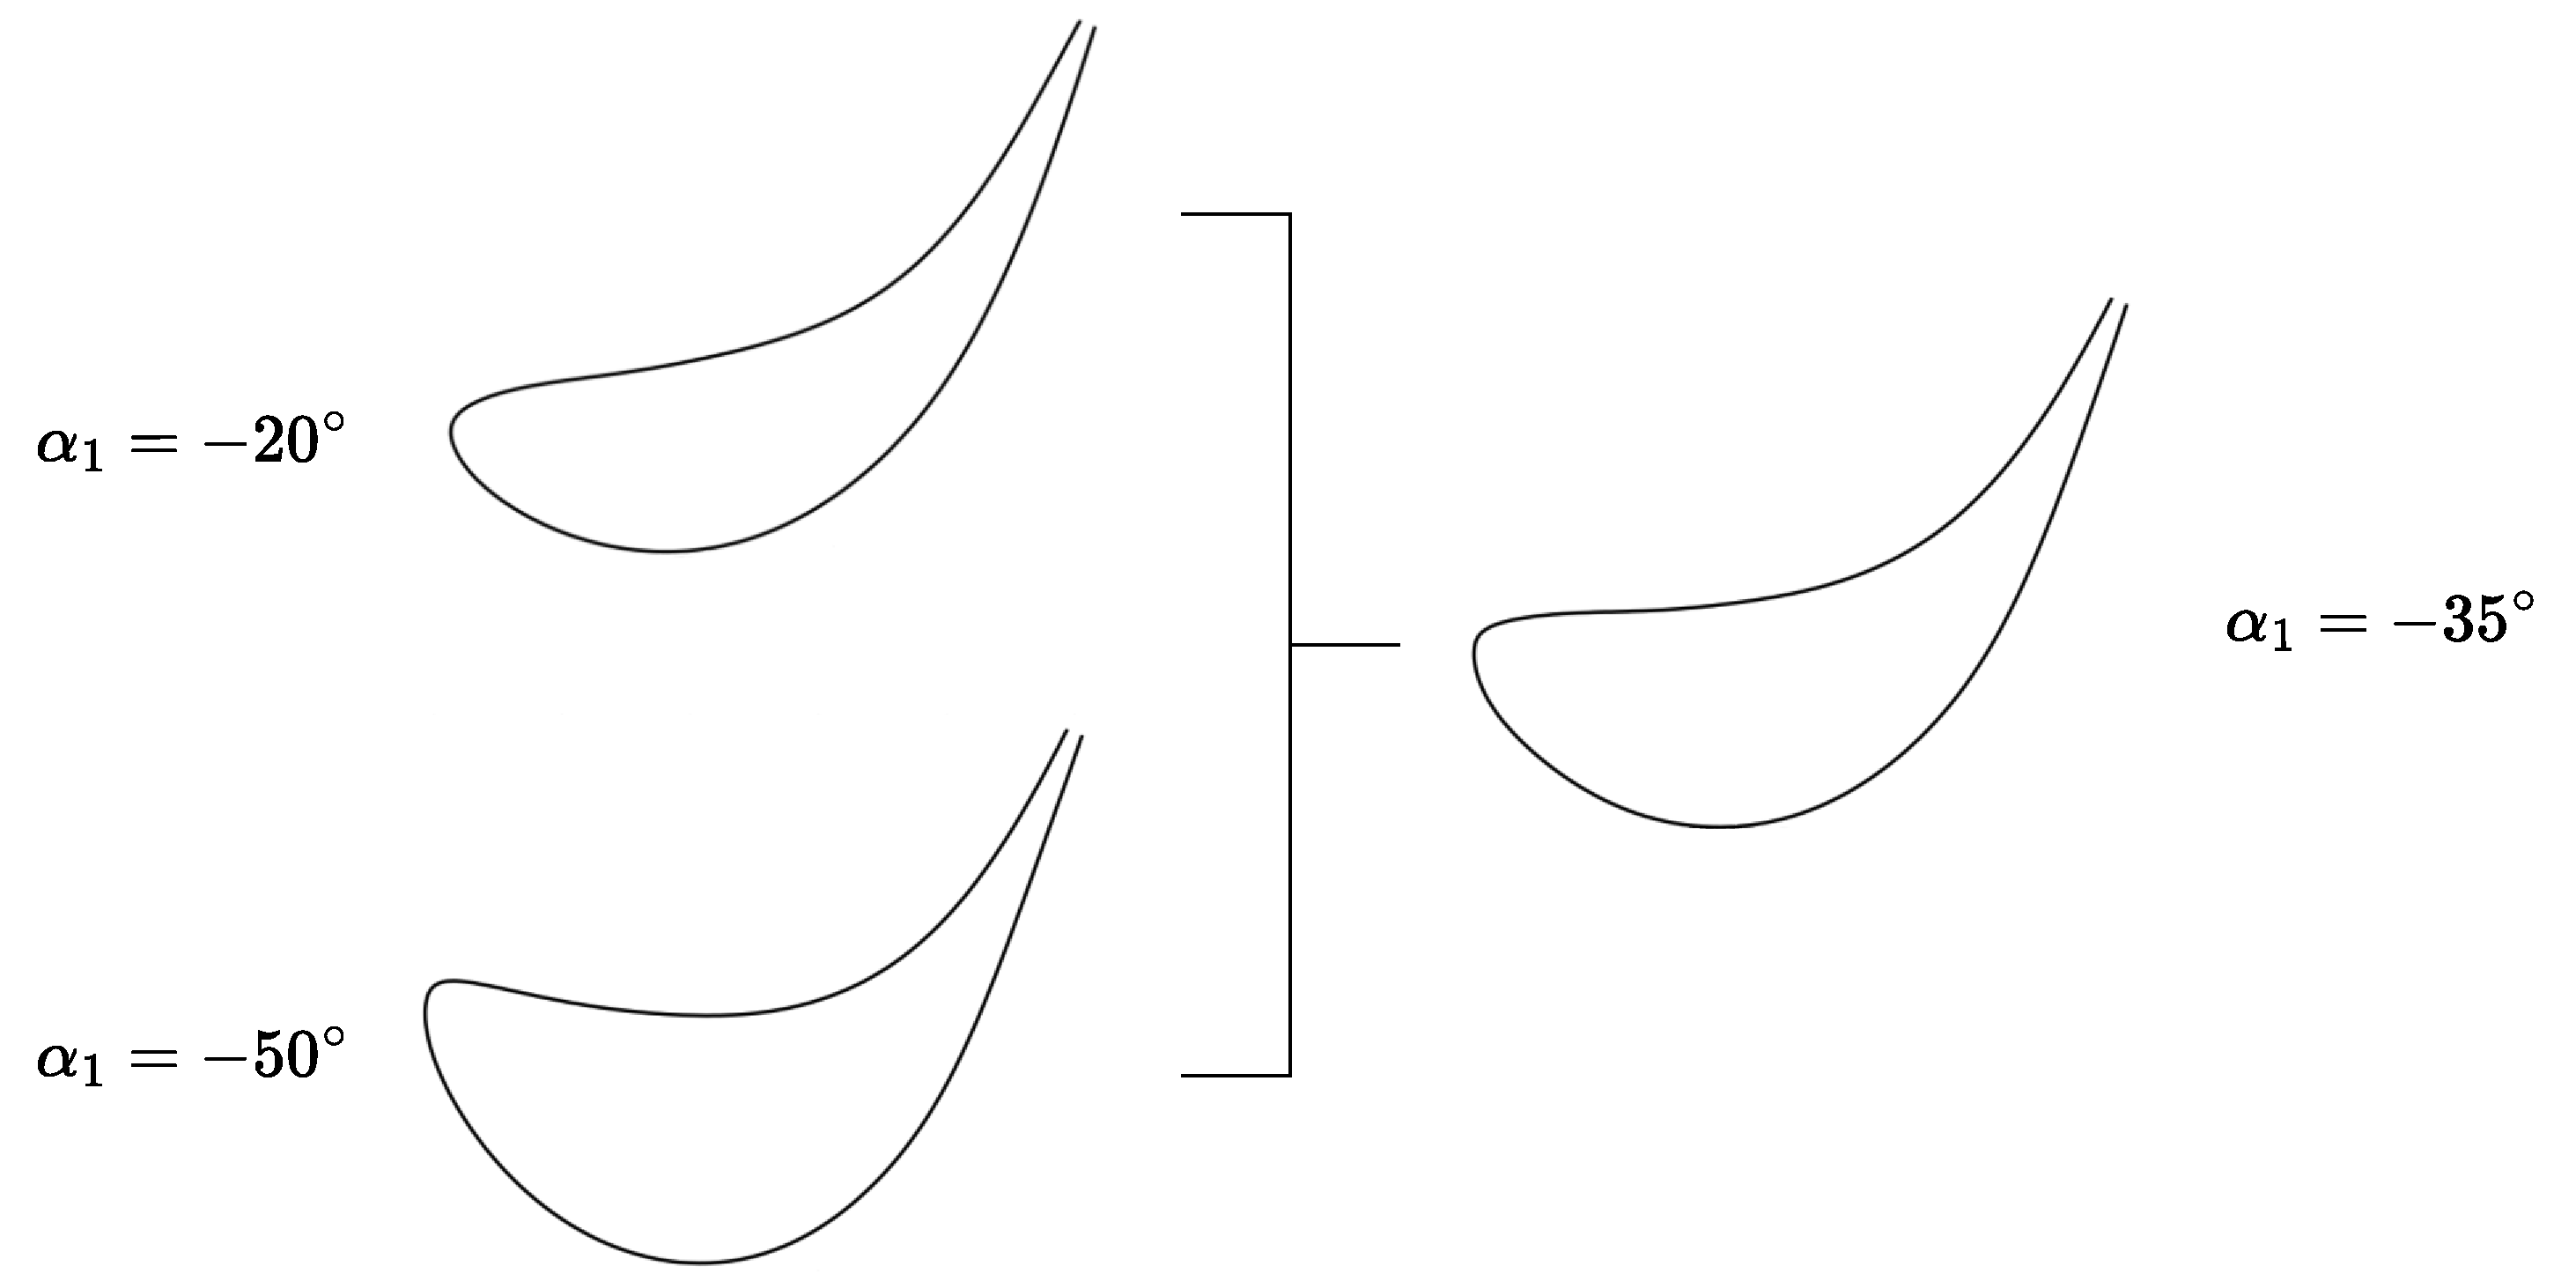
\includegraphics[page=1, scale=0.2]{./pdf/innerGeometry.pdf}
    \end{figure}
    From this guess, a \textbf{new optimization} of the inner point is made.
\end{frame}

\begin{frame}{Objectives \& constraints}
    \begin{columns}
        \column{0.5\textwidth}
            \begin{center}
                \renewcommand{\arraystretch}{2}
                \begin{tabularx}{1\textwidth} { 
                    || >{\centering\arraybackslash}X 
                    | >{\centering\arraybackslash}X 
                    | >{\centering\arraybackslash}X 
                    | >{\centering\arraybackslash}X || } 
                    \hline
                    Obj. & Min & Max & Points\\ [0.5ex] 
                    \hline\hline
                    $\frac{M_P}{M_{TE}}$ & $1.2$ & $1.4$ & 3 \\ [0.5ex]
                    \hline
                    $\frac{L_P}{L_{surf}}$ & $0.5$ & $0.6$ & 3 \\ [0.5ex]
                    \hline
                    $\frac{M_{LE}}{M_{TE}}\frac{M_2}{M_1}$ & $1.2$ & $1.8$ & 3 \\ [0.5ex]
                    \hline
                    $\frac{M_{PS}}{M_{TE}}\frac{M_2}{M_{1, ax}}$ & $0.8$ & $1.2$ & 3 \\ 
                    \hline
                \end{tabularx}
            \end{center}
        \column{0.5\textwidth}
            \begin{center}
                \renewcommand{\arraystretch}{2}
                \begin{tabularx}{1\textwidth} { 
                    || >{\centering\arraybackslash}X 
                    | >{\centering\arraybackslash}X 
                    | >{\centering\arraybackslash}X 
                    | >{\centering\arraybackslash}X || } 
                    \hline
                    Constr. & Min & Max & Points\\ [0.5ex] 
                    \hline\hline
                    $\alpha_1$ & $-50^{\circ}$ & $-20^{\circ}$ & 3 \\ [0.5ex]
                    \hline
                    $\alpha_2$ & $65^{\circ}$ & $72.5^{\circ}$ & 4 \\ [0.5ex]
                    \hline
                    $M_2$ & $0.4$ & $0.7$ & 3 \\ [0.5ex]
                    \hline
                    $Re$ & $6 \cdot 10^5$ & $6 \cdot 10^5$ & 1 \\ 
                    \hline
                \end{tabularx}
            \end{center}
    \end{columns}
\end{frame}